\begin{pastexam}[label={px:ntu-106-esoe-ds-03}]{臺大工科海洋所 106 學年度 第 3 題}
（問答）

\textbf{(10 \%)} What does the following minimum binary heap look like after removeMin( )?
\begin{center}
\begin{tabular}{|c|c|c|c|c|c|c|c|c|c|}\hline
$\times$ & 1 & 4 & 3 & 5 & 4 & 15 & 9 & 16 & 8\\\hline
\end{tabular}
\end{center}
\end{pastexam}

\begin{pastsoln}
答案：$[\times, 3, 4, 8, 5, 4, 15, 9, 16]$。

第 $0$ 格打叉表示不用，堆積從第 $1$ 格開始存，$A[i]$ 的子節點是 $A[2i]$、$A[2i+1]$（資結書
第~7.2.1~節）。 原本的堆積：
\begin{center}
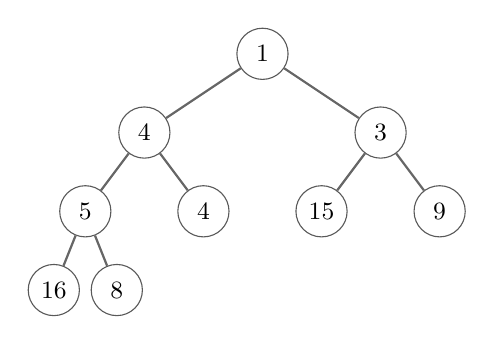
\begin{tikzpicture}[
    btn/.style={circle, draw=black!65, line width=0.4pt, minimum size=6.5mm, inner sep=0pt, font=\small},
    level distance=10mm, edge from parent/.style={draw=black!60, thick},
    level 1/.style={sibling distance=30mm}, level 2/.style={sibling distance=15mm},
    level 3/.style={sibling distance=8mm}]
\node[btn] {1}
    child {node[btn] {4}
        child {node[btn] {5} child {node[btn] {16}} child {node[btn] {8}}}
        child {node[btn] {4}}}
    child {node[btn] {3}
        child {node[btn] {15}}
        child {node[btn] {9}}};
\end{tikzpicture}
\end{center}
先確認它真的是最小堆積：$1 \le 4, 3$；$4 \le 5, 4$；$3 \le 15, 9$；$5 \le 16, 8$，每個父節點都
不大於子節點。

removeMin 的做法（資結書第~8.1~節虛擬碼~8.2）：取出根 $1$，把最後一格的 $8$ 搬到根，堆積
大小從 $9$ 變成 $8$，再從根往下調整（sift-down）：每次和比較小的子節點比，子節點比較小就交換。
\begin{center}
\begin{tabular}{lll}
\toprule
步驟 & 比較 & 陣列 $A[1..8]$ \\
\midrule
取出 $1$，$8$ 搬到根 & & $8, 4, 3, 5, 4, 15, 9, 16$ \\
$8$ 在第 $1$ 格 & 子節點 $4$、$3$，較小的是 $3$，$3 < 8$，交換 & $3, 4, 8, 5, 4, 15, 9, 16$ \\
$8$ 在第 $3$ 格 & 子節點 $15$、$9$，較小的是 $9$，$9 > 8$，停 & $3, 4, 8, 5, 4, 15, 9, 16$ \\
\bottomrule
\end{tabular}
\end{center}
結果（被取出的最小值是 $1$）：
\begin{center}
\begin{tabular}{|c|c|c|c|c|c|c|c|c|}\hline
$\times$ & 3 & 4 & 8 & 5 & 4 & 15 & 9 & 16\\\hline
\end{tabular}
\qquad
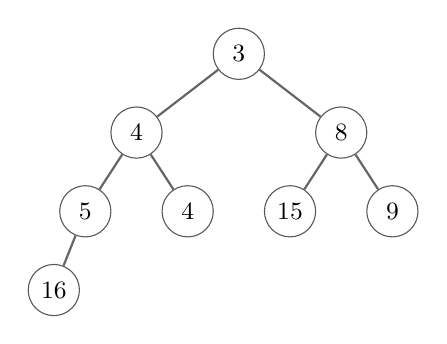
\begin{tikzpicture}[baseline=(r.center),
    btn/.style={circle, draw=black!65, line width=0.4pt, minimum size=6.5mm, inner sep=0pt, font=\small},
    level distance=10mm, edge from parent/.style={draw=black!60, thick},
    level 1/.style={sibling distance=26mm}, level 2/.style={sibling distance=13mm},
    level 3/.style={sibling distance=8mm}]
\node[btn] (r) {3}
    child {node[btn] {4}
        child {node[btn] {5} child {node[btn] {16}} child[missing]}
        child {node[btn] {4}}}
    child {node[btn] {8}
        child {node[btn] {15}}
        child {node[btn] {9}}};
\end{tikzpicture}
\end{center}
常見的錯誤是把 $8$ 和左邊的 $4$ 交換：要和\textbf{比較小}的子節點交換，否則換上來的 $4$ 會比
右子節點 $3$ 大，違反堆積性質。
\end{pastsoln}
